The state adapter uses the state completeness model to determine whether an abstract high-level state blocks or can be advanced to the next HLPC on its path.
%
\chef provides two completeness models: \emph{partial} and \emph{complete}.
%
The two models provide different trade-offs between the precision of controlling the high-level execution and the expected path throughput in the high-level symbolic execution engine.

\begin{figure}
  \centering
  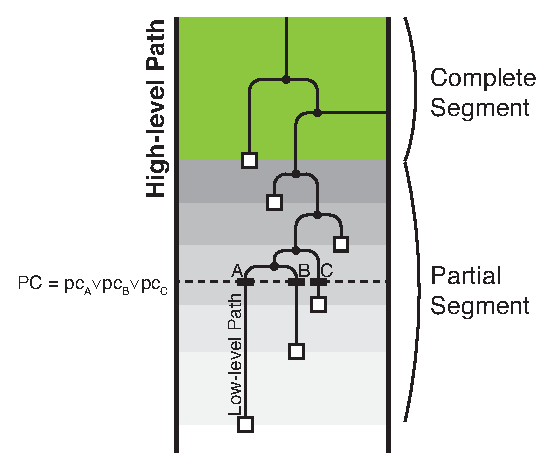
\includegraphics[width=3in]{chef/figures/path-segments}
  \caption{High-level execution path, segmented according to completeness of exploration by the low-level paths.}
  \label{fig:chef:path-segments}
\end{figure}

Before we present the two models, we introduce the notion of \emph{local path condition} and \emph{path segments} (Figure~\ref{fig:chef:path-segments}).

\paragraph{Local Path Condition}

We define the local path condition of a high-level path at a given HLPC location as the disjunction of the path conditions of all low-level states that traversed the HLPC location, \emph{at the moment the interpreter started executing the statement at the given HLPC}.
%
Each statement on the high-level path has a local path condition.

The local path condition of a HLPC location is \emph{complete} if all low-level states on the path are located after the statement.
%
This means that there is no further interpreter execution that would reach the HLPC location.
%
Hence, a complete local path condition describes \emph{all} inputs that take the program along the given high-level path.

Conversely, if there exist low-level states that are located before the HLPC location on the path, its local path condition is \emph{partial}.
%
The local path condition shown in Figure~\ref{fig:chef:path-segments} is partial, because there are three states before it.
%
Any of them could reach the program at that location and augment the possible program executions on the path.

\paragraph{Path Segments}

We divide a high-level execution path in two segments, according to the completeness of the local path conditions of its HLPC locations:
\begin{itemize}
\item The \emph{complete segment} consists of all locations traversed by all low-level states on the path.
%
The segment starts at the beginning of the path and ends at the HLPC of the least advanced low-level state on the path (the green block in Figure~\ref{fig:chef:path-segments}).
\item The \emph{partial segment} consists of the rest of the path, which contains the locations traversed by at least one, but not all, low-level states on the path.
%
The segment starts with the least advanced low-level state on the path and ends at the leading state on the path.  Figure~\ref{fig:chef:path-segments} shows the partial segment in nuances of gray, according to the degree of local path completeness.
\end{itemize}

Each HLPC location on the high-level path transitions from partial to complete.
%
In case a high-level path consists of a single low-level path, the transition goes directly to complete and the partial segment is empty.

\paragraph{The State Completeness Models}

The partial and completeness models are defined with respect to the path segments on which the abstract high-level states are allowed to reside.

In the partial model, the abstract high-level states are allowed to reside anywhere on the high-level execution path, i.e., on both its complete and partial segment.
%
On the other hand, in the complete model, the abstract high-level states are only allowed on complete segments.

This difference creates substantial divergences in the properties of the two models, which we discuss next.

\subsection{Partial High-level Execution States}

In the partial model, the abstract high-level states are allowed to reside anywhere on the high-level execution path.
%
Therefore, the states block only at the last HLPC location on the path.

The low-level strategy unblocks the abstract high-level states by selecting for execution the leading low-level state on the path.
%
Therefore, the cost of unblocking the state is relatively low: only one low-level state from the entire path is required, which amounts to simpler symbolic expressions and faster solver queries.

On the other hand, in the partial model, the execution of the abstract high-level state may miss feasible high-level branches.
%
This is because the local path condition of the abstract state is incomplete, and therefore may not include the low-level executions that diverge into other high-level paths at branching points.
% GIVE EXAMPLE
% For interpreted languages, many instructions can potentially be branching points, either as explicit branch instructions, or as statements that may throw exceptions.

As a result, the high-level strategy can only exercise control over high-level paths \emph{already discovered}.
%
New high-level paths are discovered only as the low-level strategy repeatedly selects low-level states for execution on the existing paths.


\subsection{Complete High-level Execution States}

In the complete model, the abstract high-level states can only reside on the complete path segment.
%
The states block at the first low-level state encountered on the path, before entering the partial segment.

The low-level strategy unblocks the abstract high-level states by executing all low-level states that reside on the next statement on the path.
%
Therefore, compared to the partial mode, the cost of unblocking the state is significantly higher.

However, in the complete model, the feasibility of all branching instructions traversed by the abstract high-level states are decided, as the local path conditions are complete.
%
In turn, the high-level execution strategy has knowledge of all paths forking off the currently discovered ones, and can influence the exploration ordering.

\subsection{Choosing Between the Two Models}

\newcommand{\goodcolor}{\cellcolor{LimeGreen}}
\newcommand{\badcolor}{\cellcolor{Lavender}}

\begin{table}
  \centering
  \small
  \begin{tabular}{r c c}
    High-level State Model & \textbf{Partial} & \textbf{Complete}               \\
    \hline
    \noalign{\smallskip}
    Location (HLPC) & Complete and partial segments & Complete segments only    \\
    Path Condition  & Incomplete                    & Complete                  \\
    Strategies      & Only at low level             & Both high- and low-level  \\
    \noalign{\smallskip}
    \hline
    \noalign{\smallskip}
    Efficiency (state cost) & \goodcolor One low-level state   & \badcolor All low-level states      \\
    Precision       & \badcolor Low (no branch feasibility)   & \goodcolor Full control over states  \\
  \end{tabular}
  \caption{Comparing partial and complete high-level state models in \chef.}
  \label{tab:chef:hl-states}
\end{table}

Table~\ref{tab:chef:hl-states} summarizes the trade-offs between the partial and complete state models.
%
On the one hand, the partial state model lacks precision, as it does not expose to the high-level engine interface any pending high-level states, but gains efficiency, as it uses as little as one low-level state to explore a high-level path, once discovered.
%
On the other hand, the complete state model provides full precision, as it is able to determine all feasible branches along each explored path, at the expense of a more costly path exploration.

Both state models are useful for symbolic execution.
%
Fundamentally, both models handle the same low-level state information coming from the underlying symbolic execution engine.  The difference relates to how the data is organized into execution paths and test cases.

The partial state model works best for exploratory automated test case generation.
%
The low-level strategy aims to discover new high-level paths, which are then executed efficiently using a single low-level state, which gives the test case for the path.

The precise state model is more appropriate for directed test case generation and exhaustive testing.
%
The high-level strategy works with the low-level strategy to focus the exploration on particular high-level paths.  At the same time, the decoupling between the two strategies opens up optimization opportunities at the low-level, such as state merging, which increases the efficiency of exhaustive testing.

%% This limitation makes it more difficult to build analyses that read the program state, including search selection strategies, such as the coverage-optimized strategy in \klee~\cite{klee}.
%% %
%% However, the high-level state remains implicitly encoded in the low-level interpreter state and can be accessed by executing code in the target language, by the interpreter runtime.  Therefore, a possible workaround is to split the analysis in a language-independent part, running as part of Chef, and a language-dependent part, written in the target language and running as an interrupt in the interpreter context, whenever it is needed.

%% Determining the positions of a high-level state on its high-level path is not as clear-cut.
%% %
%% The low-level states on the high-level path may reside at different points on the path, so there is no straightforward mapping from them to the high-level state.

%% The leading low-level state of the high-level path defines the boundary between the partial and undiscovered segment, while the trailing state on the path defines the boundary between the completed and partial segment.

%% %
%% In other words, the goal of the system becomes that of maximizing the high-level path yield for the set of low-level paths explored.
%
%% However, as executing low-level paths is efficient, in practice, a judicious state selection strategy can effectively discover significantly more high-level paths compared to naively choosing paths at random (Section~\ref{sec:xxx}).


%%% Local Variables: 
%%% mode: latex
%%% eval: (visual-line-mode)
%%% fill-column: 1000000
%%% TeX-master: "main"
%%% End:
